% =====================
\section{Tools and Libraries for Face Recognition}

In this project, a combination of custom model creation and pre-built libraries was utilized for face detection and recognition. This section provides an overview and comparison of the main tools and algorithms employed.

\subsection{Custom Model Creation}

\textbf{OpenCV:} Used for image processing and face detection via Haar cascades, which are trained classifiers for detecting facial features.

\textbf{TensorFlow:} The deep learning model was built using TensorFlow, focusing on convolutional neural networks (CNNs) for feature extraction and classification.

\textbf{Albumentations:} Applied for data augmentation, introducing variations such as brightness, contrast, rotation, and noise to improve model robustness.

\textbf{Labelme:} Used for manual annotation of facial regions, providing high-quality labels for supervised training.

\textbf{Algorithms:}
\begin{itemize}
    \item \textbf{Haar Cascades (OpenCV):} Real-time face detection using edge and feature detection.
    \item \textbf{Convolutional Neural Networks (TensorFlow):} Feature extraction and classification for face recognition.
    \item \textbf{Data Augmentation:} Enhances dataset diversity and model generalization.
\end{itemize}

\begin{figure}[ht!]
    \centering
    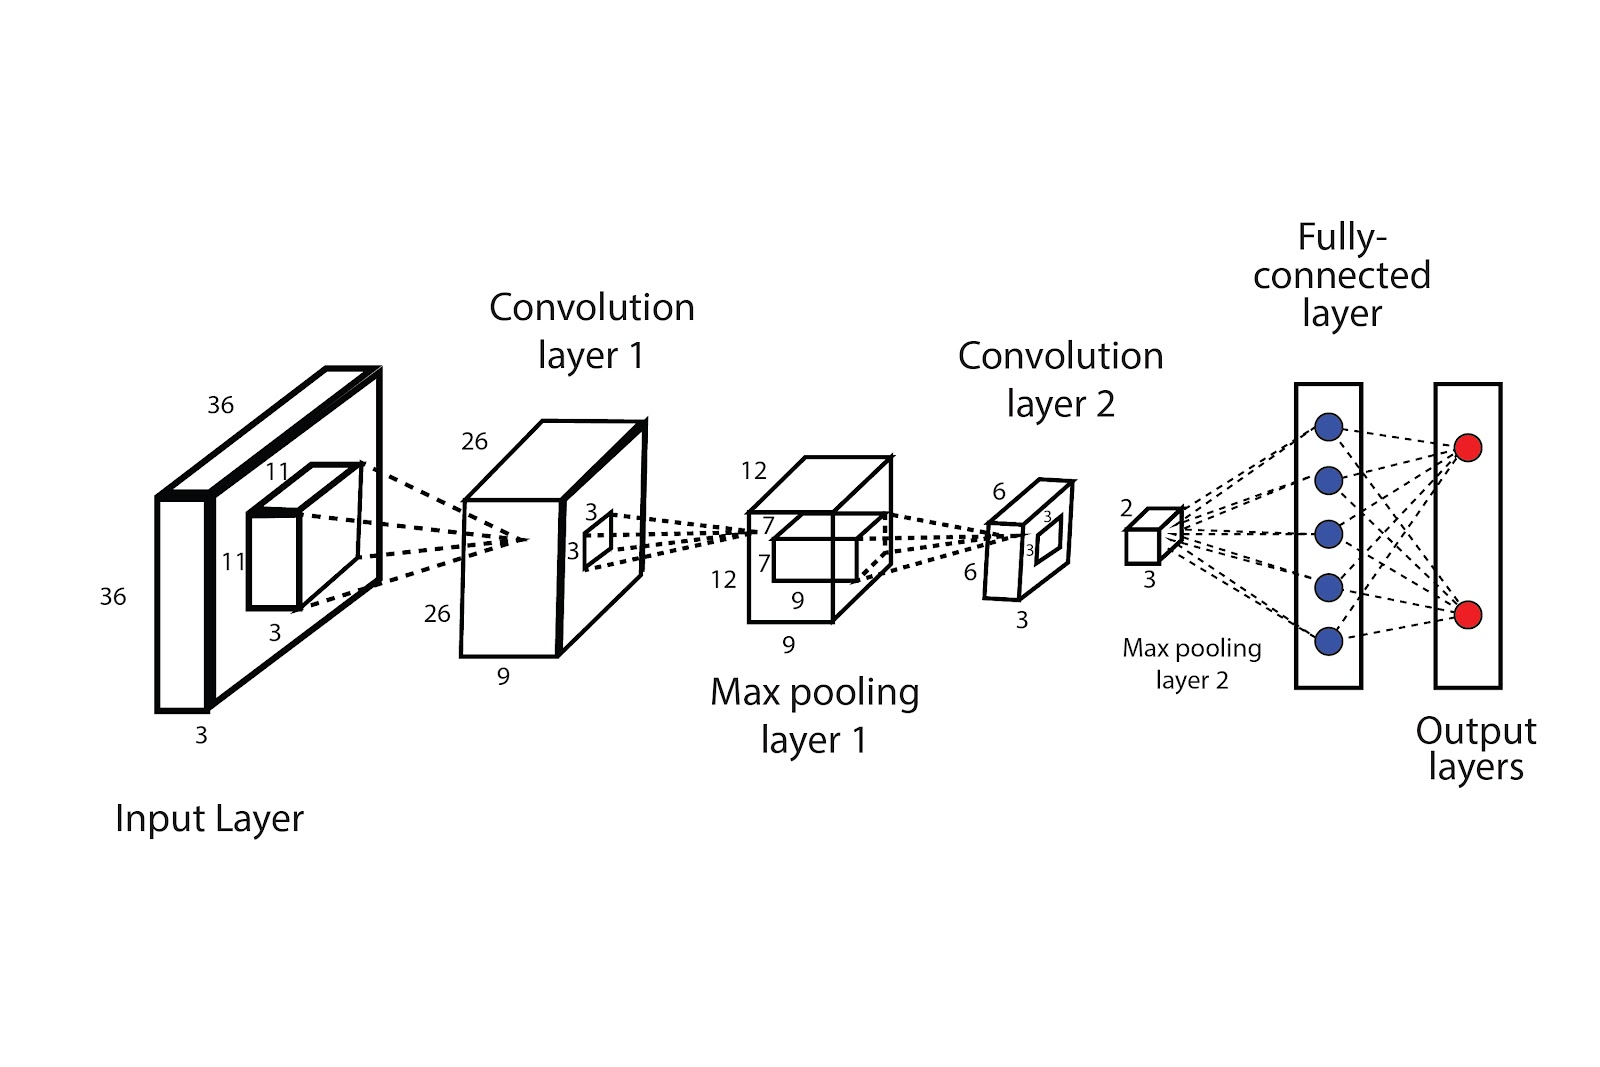
\includegraphics[width=0.7\textwidth]{../Files/convolutional_network_architecture.png}
    \caption{Architecture of the convolutional neural network used in the custom model.}
    \label{fig:cnn-architecture}
\end{figure}

\subsection{face-recognition Library}

\textbf{dlib:} Provides face detection (HOG) and recognition (ResNet-34 based deep metric learning).

\textbf{face\_recognition:} Python wrapper for dlib, simplifying face detection and recognition.

\textbf{OpenCV:} Used for image preprocessing.

\textbf{Algorithms:}
\begin{itemize}
    \item \textbf{Histogram of Oriented Gradients (HOG):} Robust face detection across lighting conditions.
    \item \textbf{Deep Metric Learning (ResNet-34):} Encodes faces into 128-dimensional vectors for comparison.
\end{itemize}

\begin{figure}[ht!]
    \centering
    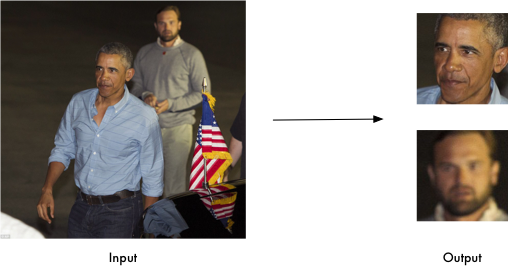
\includegraphics[width=0.7\textwidth]{../Files/face_recognition_example.png}
    \caption{Example of face recognition using the face\_recognition library.}
    \label{fig:face-recognition-example}
\end{figure}

\subsection{MTCNN (Multi-task Cascaded Convolutional Networks)}

MTCNN is a deep learning-based framework for face detection and landmark localization, using a cascade of three neural networks (P-Net, R-Net, O-Net) for robust detection and alignment.

\subsection{FaceNet}

FaceNet maps faces into a Euclidean space using a deep CNN and triplet loss, enabling verification, clustering, and identification. It is implemented with TensorFlow or PyTorch and uses Inception networks for feature extraction.

\subsection{Amazon Rekognition}

Amazon Rekognition is a cloud-based service for face detection, recognition, and analysis, using proprietary deep learning algorithms. It offers face comparison, attribute analysis, and is widely used in security and media applications.

\subsection{References}
\begin{itemize}
    \item Comparison of deep learning software: \url{https://en.wikipedia.org/wiki/Comparison_of_deep_learning_software}
    \item TensorFlow Documentation: \url{https://www.tensorflow.org/}
    \item OpenCV Python Documentation: \url{https://docs.opencv.org/4.x/}
    \item Albumentations Documentation: \url{https://albumentations.ai/docs/}
    \item Face Recognition Documentation: \url{https://pypi.org/project/face-recognition/}
    \item dlib Documentation: \url{http://dlib.net/}
    \item Zhang, K., et al. (2016). Joint face detection and alignment using multitask cascaded convolutional networks. IEEE Signal Processing Letters, 23(10), 1499-1503.
    \item Schroff, F., et al. (2015). FaceNet: A unified embedding for face recognition and clustering. In Proceedings of the IEEE Conference on Computer Vision and Pattern Recognition (pp. 815-823).
    \item Amazon Rekognition Developer Guide: \url{https://docs.aws.amazon.com/rekognition/}
\end{itemize}

% =====================
\section{Methods and Algorithms for Face Recognition}

Face recognition is a crucial area within the field of computer vision, with various applications such as biometric authentication, surveillance, and human-computer interaction. Over the years, researchers have developed numerous techniques to accurately identify and verify faces in images. In this chapter, we explore some of the most prominent methods and algorithms used for face recognition, focusing on their theoretical aspects.

\subsection{Convolutional Neural Networks (CNNs)}
Convolutional Neural Networks (CNNs) are perhaps the most widely used algorithm for face recognition today. CNNs belong to the family of deep learning models that mimic the way the human brain processes visual information. Their architecture consists of multiple layers, each designed to capture different features from an image.

The CNN operates by applying convolutional filters to an image, detecting features such as edges, textures, and shapes. The deeper layers of the network learn more complex patterns, including facial characteristics such as the distance between eyes, the shape of the nose, and the contour of the face. CNNs are well-suited for face recognition because of their ability to extract hierarchical features that capture both local and global information from an image.

Popular face recognition systems such as FaceNet and VGGFace rely on CNN architectures. These models are trained on large datasets containing millions of labeled faces, enabling them to generalize across different lighting conditions, angles, and facial expressions. CNNs are typically employed in combination with classification or embedding techniques for face verification and identification tasks.

\subsection{Eigenfaces}
The Eigenface method is a classical approach based on Principal Component Analysis (PCA). Developed in the early 1990s~\cite{turk1991eigenfaces}, this method represents faces as linear combinations of a set of basis images known as ``eigenfaces.'' Each eigenface corresponds to a direction of maximal variance in the face dataset. The idea behind this method is to reduce the dimensionality of face data while retaining the most significant information that differentiates one face from another.

To recognize a face using the Eigenface approach, an input image is projected onto the subspace spanned by the eigenfaces. The resulting projection is compared to stored projections of known faces in the database. Recognition is achieved by measuring the similarity between the input face's projection and the stored ones~\cite{alochana_study_2024}.

Turk and Pentland reported recognition rates of 96\% for lighting variations, 85\% for orientation, and 64\% for scale variations on a dataset of 16 subjects~\cite{turk1991eigenfaces}. While fast and straightforward, Eigenfaces are highly sensitive to variations in lighting, pose, and occlusion, often requiring extensive preprocessing for image normalization to achieve optimal performance~\cite{alochana_study_2024, geeksforgeeks_ml_2021}.

\subsection{Fisherfaces}
Fisherfaces improve upon Eigenfaces by using Linear Discriminant Analysis (LDA) rather than PCA. While PCA focuses on maximizing the variance in the data, LDA aims to maximize the class separability, which makes Fisherfaces more robust to variations within the same class (such as different expressions of the same individual).

The Fisherface approach projects the face data onto a subspace where the ratio of the between-class scatter to the within-class scatter is maximized. This results in a set of features that better discriminates between different individuals, even under varying lighting conditions or facial expressions.

Fisherfaces, therefore, offer better performance than Eigenfaces, especially in more realistic, variable conditions, making it a more practical choice for face recognition.

\subsection{Local Binary Patterns (LBP)}
Local Binary Patterns (LBP) is a texture-based method used for facial feature extraction. The algorithm works by dividing the face into small regions and calculating a binary pattern based on the relative intensity of the neighboring pixels. Each region is then represented by a histogram of these binary patterns, which collectively form a feature vector that can be used for face recognition.

The advantage of LBP lies in its simplicity and computational efficiency. It is also robust to changes in lighting, which makes it well-suited for real-time face recognition in low-power or resource-constrained environments. LBP has been successfully used in various face recognition tasks and is particularly useful for recognizing faces in surveillance systems.

\subsection{Haar Cascades}
The Haar Cascade classifier, introduced by Paul Viola and Michael Jones in 2001, is another widely used algorithm for face detection and recognition. This method is based on the concept of Haar-like features, which are used to detect objects in images by analyzing the contrast between adjacent areas.

The Haar Cascade algorithm works by applying a series of rectangular features to different regions of the image. It uses an integral image representation to compute these features efficiently, allowing for rapid detection. The key to Haar Cascades is the cascade classifier, which consists of multiple stages of increasingly complex classifiers. Each stage eliminates non-face regions, progressively narrowing down the areas that are likely to contain faces.

Although Haar Cascades are primarily used for face detection, they can also be employed for face recognition when combined with other methods like PCA or LBP. Haar Cascades are lightweight and fast, making them ideal for real-time applications, though they tend to perform poorly in unconstrained environments.

\subsection{Histogram of Oriented Gradients (HOG)}
The Histogram of Oriented Gradients (HOG) method is a feature extraction technique that captures the gradient orientation and intensity within an image. It is commonly used for object detection, including face recognition. The HOG algorithm divides the face into small cells and computes a histogram of gradient directions for each cell. These histograms are then concatenated to form a feature descriptor representing the face.

HOG-based face recognition is robust to small variations in pose and lighting, and it is computationally efficient. However, its performance is generally lower than deep learning-based approaches like CNNs, especially when dealing with more complex, unconstrained face recognition tasks.

\subsection{Deep Metric Learning}
Deep Metric Learning is an advanced technique used for face recognition tasks that involve face verification or identification. The core idea of metric learning is to map faces into an embedding space, where the distance between vectors represents the similarity between faces. The most well-known example of this approach is the FaceNet model, which uses a triplet loss function to ensure that faces of the same person are closer together in the embedding space than faces of different people.

This technique enables robust face recognition by transforming the problem into a similarity comparison rather than a direct classification task. Deep Metric Learning is highly effective in handling large-scale face recognition problems with varying conditions, and it has become a key method for many modern face recognition systems.

\subsection{3D Face Recognition}
3D face recognition methods use the three-dimensional geometry of the human face to improve recognition accuracy, especially in cases where 2D methods may struggle, such as with changes in lighting, pose, or facial expression. These methods involve capturing 3D data using sensors like structured light or time-of-flight cameras. The 3D face model allows for a more detailed representation of the face's surface and can be more robust to pose variations.

3D face recognition is typically combined with 2D methods to enhance performance. Although more accurate, the requirement for specialized sensors makes this approach less practical for everyday applications compared to 2D methods.

\subsection{Viola-Jones Algorithm}
Introduced in 2001, the Viola-Jones algorithm revolutionized real-time object detection, particularly for faces~\cite{wijaya_trends_2025}. It employs Haar-like features, an integral image for rapid computation, an AdaBoost classifier for feature selection, and a cascaded structure to efficiently discard non-face regions~\cite{wijaya_trends_2025}. While widely adopted due to its speed and simplicity, this framework exhibits limitations in detecting faces that are significantly occluded, improperly oriented (e.g., profile views), or subjected to substantial variations in lighting conditions~\cite{researchgate_evaluation_2023, wijaya_trends_2025}. Its training process can also be computationally intensive and time-consuming~\cite{researchgate_evaluation_2023}.